\documentclass[a4j,12pt]{jarticle}
\usepackage[dvipdfmx]{graphicx}
\usepackage{amssymb}
\usepackage{amsmath}
\usepackage{float}
\usepackage{url}
\begin{document}
\begin{center}
\thispagestyle{empty}
\vspace*{5zh}
\huge
2019年度 卒業論文\\[50pt]
{\Huge 論理的文章のアウトラインの作成を

支援するツールの開発}\\
[80pt]
\huge
指導教員 須田 宇宙 准教授\\[30pt]
千葉工業大学 情報ネットワーク学科\\[10pt]
須田研究室\\[60pt]
1632144 \hspace{70pt} 三浦 恋\\[75pt]
\end{center}
\vspace*{-2cm}
\begin{flushright} 
\huge
提出日 2020年1月30日
\end{flushright}
\large
\newpage
\pagenumbering{roman}
\tableofcontents%目次
\newpage
\pagenumbering{arabic}
\listoffigures
\thispagestyle{empty}
\clearpage
\addtocounter{page}{-1}



\newpage

\section{緒言}
%目次を作る際は\verb+\tableofcontents+ と打ちます。\\
%新しいページに区切るときは\verb+\newpage+ と打ちます

%背景
大学では論文やレポート課題などを書かなければならない大学生に対して,論理的な思考力や論理的文章作成能力の要求が高まっている.しかし,論文やレポートを書く際にアウトラインなどの事前準備をせずに文章の作成を行ってしまう学生が多く,論理的な文章にならないことが問題点として挙げられる.
そのため,レポートの書き方の指導や修正を行うライティングセンターの設置などが進められているが継続的な利用が必要とされている.

%問題点
しかし,一般に論文や小説などの長文を作成を支援するためのツールとして,アウトラインプロセッサが使用されることが多い.
これは,文章を階層的に管理することに主眼が置かれており,学生にとって主張や根拠などが明確な一貫した文章を書く力を養うためのツールではないことが問題点となっている.

%目的
そこで本研究では,主張や根拠などが明確な一貫した論文やレポートを書くため,準備段階であるアカデミックアウトラインツールを開発することを目的としている.
\newpage

\section{論文について}
\subsection{論文とは}
論文とはエッセイや小説のように自由な文章表現ではなく,一定の形式に備えた文章表現である.またテーマをもとに問題を立て,問題に対し様々な手法で分析,考察し,問題解決につながる新たな知見や検証を行い,その結果を報告するものが論文である\cite{ren1}.

\subsection{論文の書き方}
論文を書く流れとして主に4つ作業工程を繰り返し行うことで,論文を書くことができる.また,4つの工程を以下に示す.
\begin{itemize}
  \item テーマを決める
  \item 下調べを行う
  \item アウトラインの作成する
  \item 執筆する
\end{itemize}
\subsubsection{テーマを決める}
どのようなテーマの論文を書くのかを決めるため,素朴な疑問や資料を読んだ際の疑問を大切にし,論文のテーマを決めていく.またテーマが既に決まっている場合はキーワードをもとに,図や表などを使って思考を整理し,論点を見いだし下調べに入る.

\subsubsection{下調べを行う}
論文のテーマが決まった場合テーマに関しての知識を得るため,似たテーマの論文を調べ知見を広げる必要がある.文献等を調べる際は図書館での検索やデータベースによる検索や資料を収集する.また収集した資料を読み込み,疑問点などが出てきた際には2.2.1に戻りテーマについて思考の整理などを行う.論点が定まり,十分な情報が集まるまでテーマ決めと下調べを繰り返し行う.

\subsubsection{アウトラインの作成する}
下調べが終わり論文のテーマを決めることができた場合次に,作成する文章の骨組みである,アウトラインの作成を行う.紙に書き出すことやアウトラインプロセッサなどのソフトウェアを使用して,章や節で書く内容を箇条書きに近いかたちで書いていき,全体の文章構造を決めていく.また今回はwordのアウトラインの機能を使用した作成例を図\ref{fig:a}に示す.
\begin{figure}[h]
\begin{center}
 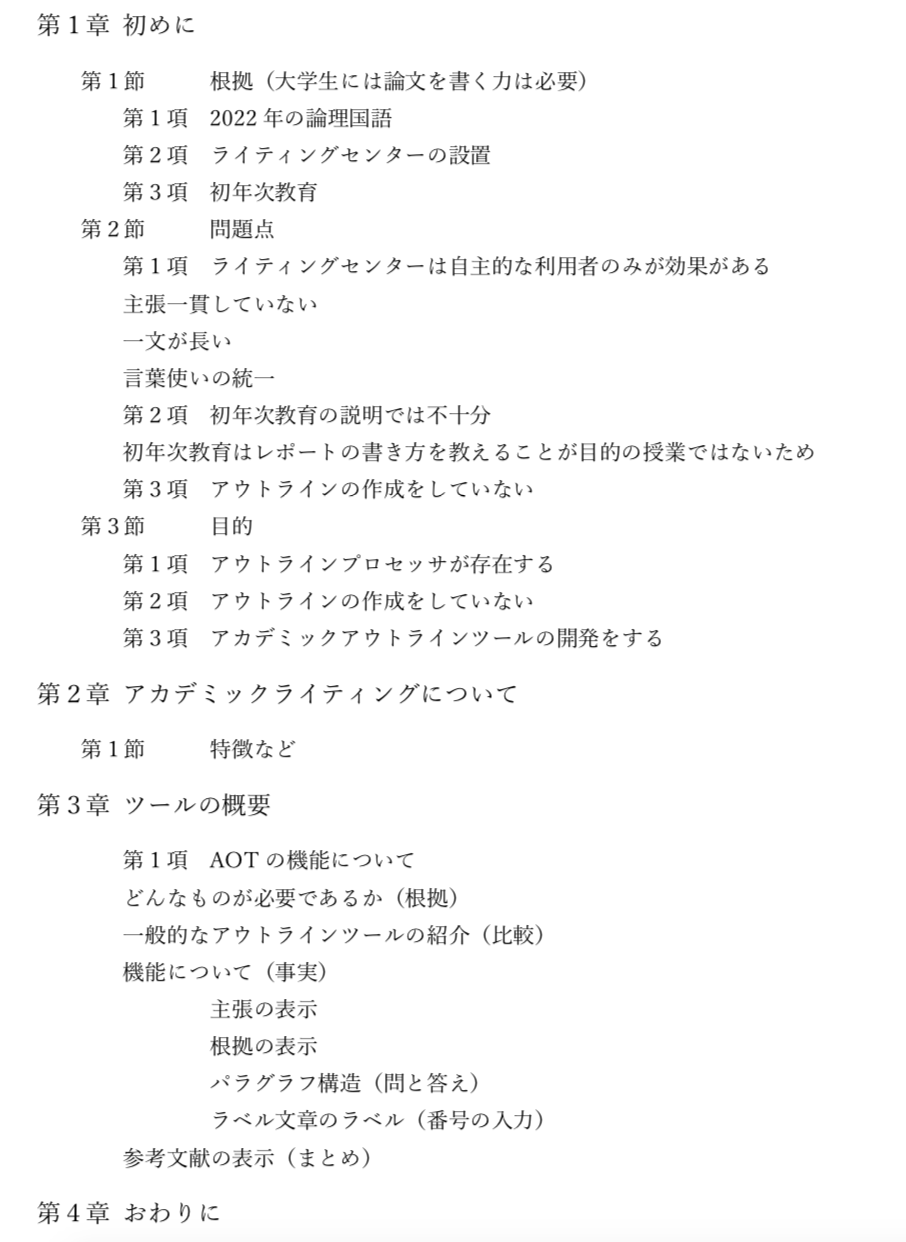
\includegraphics[clip,width=90mm,height=150mm]{outline2.png}
\end{center}
 \caption{アウトラインの作成例}
 \label{fig:a}
\end{figure}
\newpage
\subsubsection{執筆する}
フォーマットやアウトラインをもとに,執筆を行う.アウトラインや整理した資料,行った実験や検証の結果をもとにアウトラインを更に細かく作成していき,アウトラインから文章を作成をしていく.そこで必要な情報があった際には調べ,アウトラインを修正し,文章作成を行う.また,文章の書き出しから完成まで,途中何度も書いた文章を確認,添削を行う必要がある.
\newpage
\section{アカデミックライティングについて}
\subsection{アカデミックライティングとは}
大学では答えのない問題を扱い,問題に対して自分の考えを主張することが必要とされている.そこで,大学で作成が求められる論文やレポート等には複数の特徴のある文章作成が求められる.このような文章を書く技術,書く行為はアカデミックライティングと呼ばれている\cite{ren2}.
\subsection{アカデミックライティングの特徴}
アカデミックライティングには重要な特徴として,以下の(1)〜(5)が挙げられる.
\begin{description}
  \item[(1)] 主張と根拠が明示されている
  \item[(2)] 問いと答えの構造と論理的な説明での構成されている
  \item[(3)] 引用の倫理のルールに従っている
  \item[(4)] パラグラフ構造になっている
  \item[(5)] 学術的文章に特有の一定の形式に従ってる
 \end{description}
 またアカデミックライティングは,専門的な内容を論じたり,まだ答えが発見されていないことについて論じることがあるため,複雑な概念や専門用語を用いて文章の作成が行われる.しかし内容が読者に伝わらなければ文章の意味がなく,そのためにアカデミックライティングはわかりやすい文章で書く必要があることも特徴として挙げられる\cite{ren7}.
 
\newpage
\subsection{なぜアカデミックライティングが必要がなのか}
大学では答えのない問題を扱うことが多く,授業ではレポート課題が出されることがある.そこで,新たな発見を目指す研究やすでに分かっているが解釈が分かれたり,位置付けのはっきりしない事柄が多くある.そのため答えのない問題について,学生がどの程度授業の内容を理解し,また自分なりの問いや答えを見つけることに努力を行ったかを確認するために課している.

\subsection{作文・感想文との違い}
同じ文章でもアカデミックライティングは作文や感想文とは大きく異なる.作成や感想文は自分の経験や思いを書くものであり,言葉遣いも話し言葉のような文体でも許される.しかし,アカデミックライティングは文献や調査結果などの根拠をもとに学術的なルールに従った報告書である.そのため,内容として論理的な一貫した説明でなければならい.

\newpage

\section{論文などの作成を支援するソフトウェアや手法の紹介}
\subsection{アウトラインプロセッサ}
アウトラインプロセッサとは,一般的には小説などの長文を書く際に利用されている.
特徴として,見出しをつけ階層的に管理や位置の入れ替えなど行い,全体の構成を確認しながら文章の作成を支援するソフトウェアである.実際のアウトラインプロセッサの1つであるDynalistの使用例を図\ref{fig:b}に示す.
\begin{figure}[H]
\begin{center}
 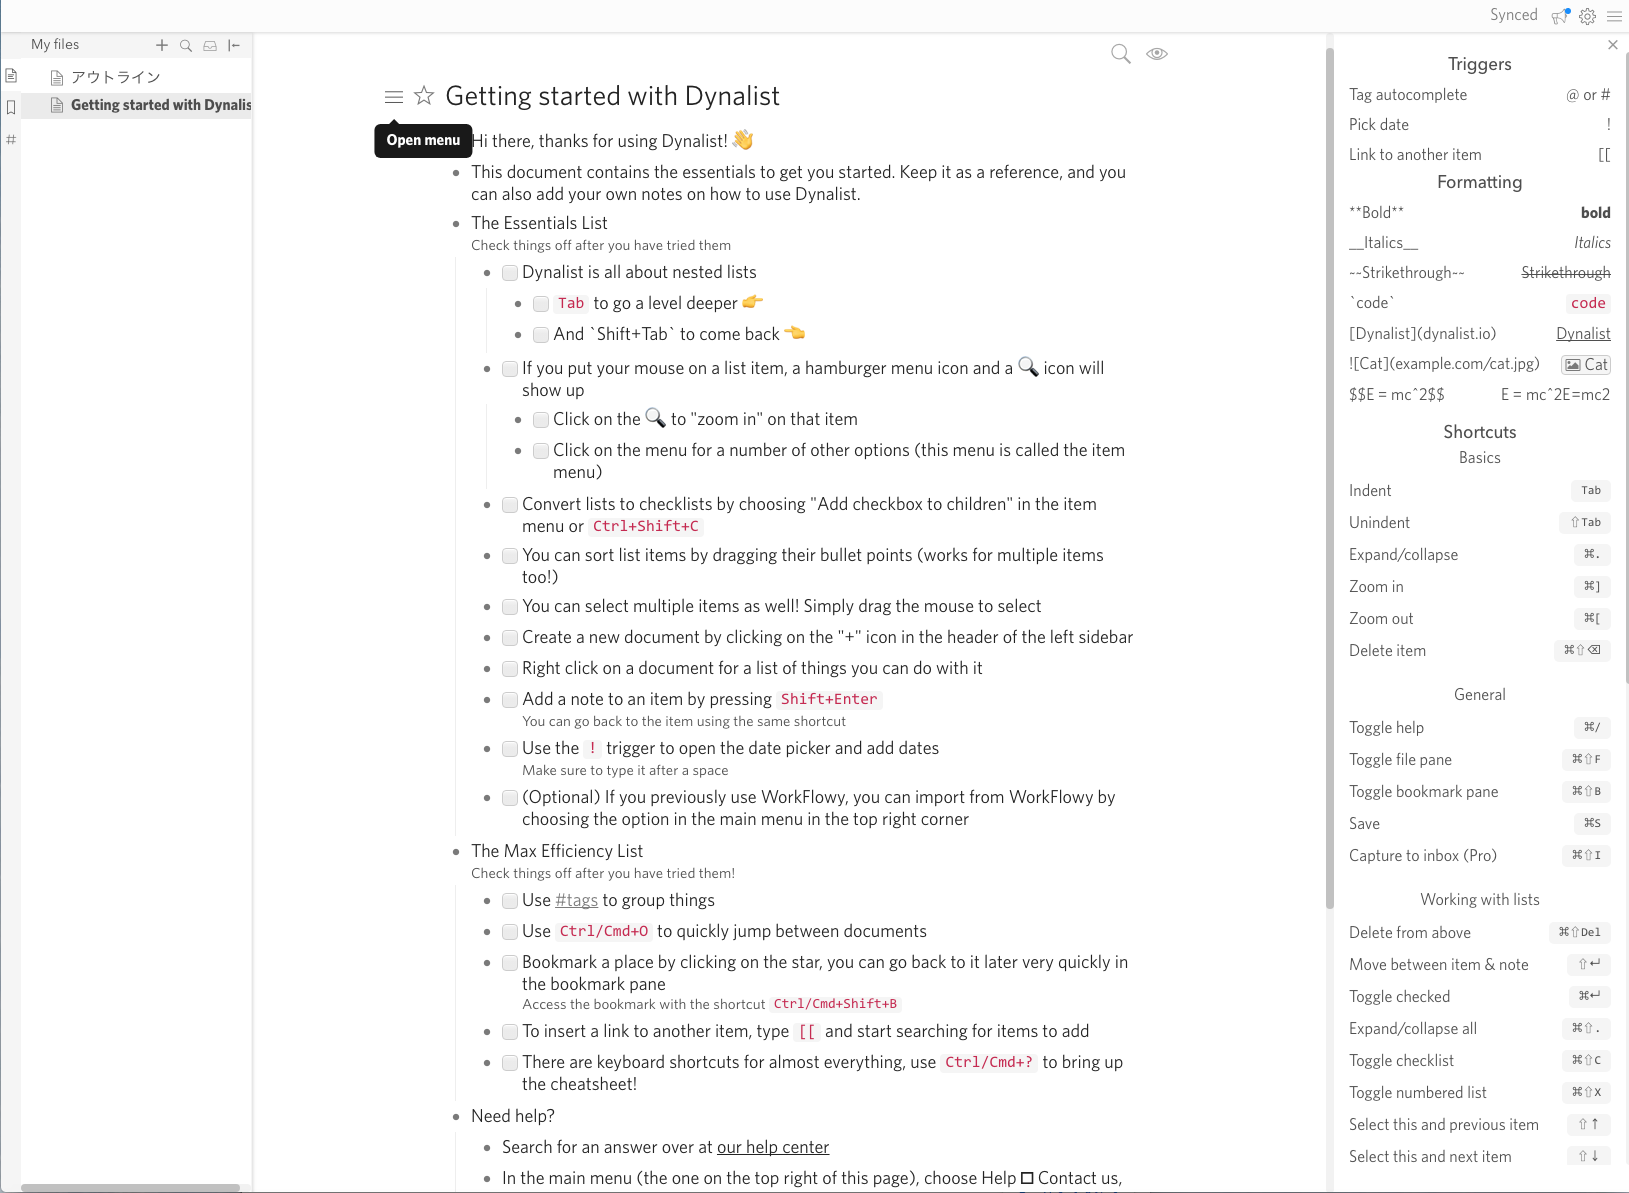
\includegraphics[clip,width=150mm,height=100mm]{Dynalist.png}
 \end{center}
 \caption{Dynalistのアウトラインの例}
 \label{fig:b}
\end{figure}
\newpage
%図の挿入をする予定
\subsection{\TeX}
\TeX とは,アメリカの著名な数学者にして計算機科学者であるDonald E. Knuthが作成した組版フリーソフトウェアである.TeX本体は,文字を配置する,基本的な組版作業に対応する命令を処理するものであり,命令だけを用いて文書を作成するのは効率的ではない.そこで多くの場合マクロセットと呼ばれる命令セットを用いて文書を作成している.

マクロとは,組版された文書の作成を容易にするために,複数の基本的な命令を組み合わせて作成された新たな命令である.
マクロセットにはさまざまなものがあるが,もっとも有名でよく用いられているものが,アメリカの計算機科学者であるLeslieLamportが作成した\LaTeX である.\TeX で文書を作成するという場合,実際はこのLaTeXの命令を用いて作成することがほとんどである.

また,日本語で書かれた文章\TeX で組版するため,(株)アスキーにおいてASCII日本語\TeX が,日本電信電話公社においてNTT J\TeX がそれぞれ開発されたことにより,日本においても\TeX が普及し現在に至っている\cite{ren3}.実際の使用例を図\ref{fig:c}に示す.

%図の挿入をする予定
\begin{figure}[H]
\begin{center}
 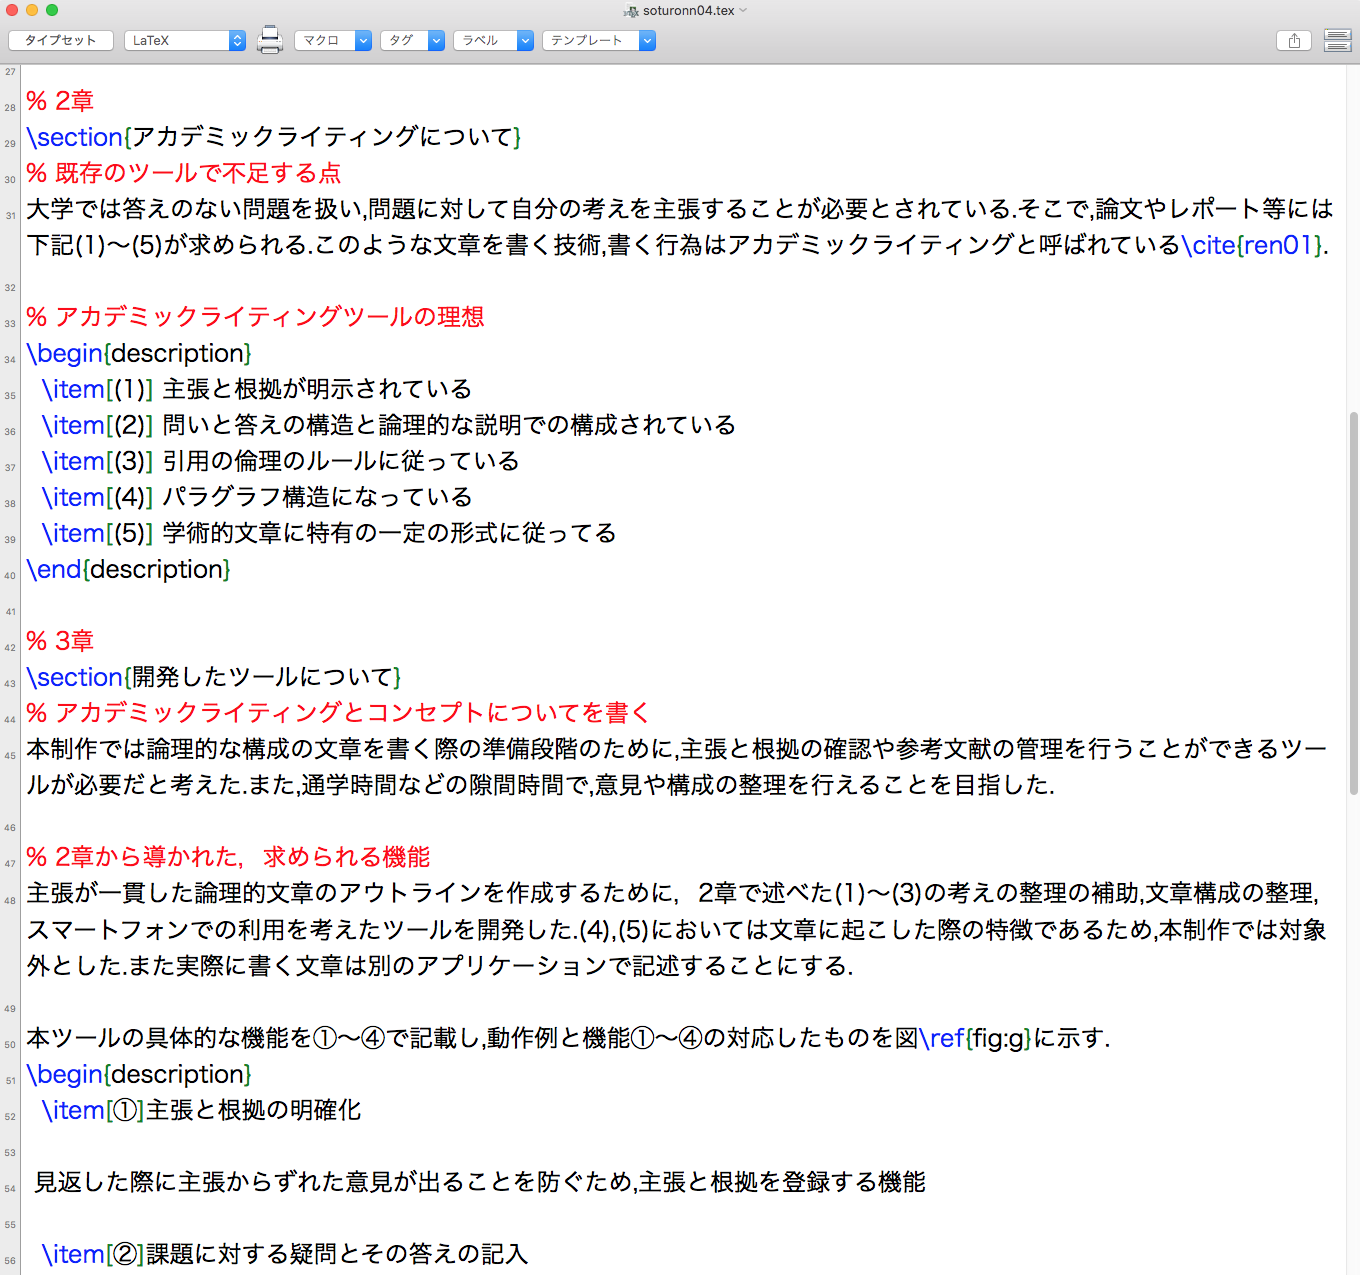
\includegraphics[clip,width=100mm,height=80mm]{TEX.png}
 \end{center}
 \caption{\TeX の使用例}
 \label{fig:c}
\end{figure}

\subsection{Microsoft Word}
WordとはMicrosoft社が提供する文章作成ソフトウェアである.Microsoft社がが販売するワープロソフトのことであり,ソフトウェアのパッケージ製品である.Microsoft Officeの中でも,主要なソフトウェアの1つに挙げられる.また,文章作成だけでなく,図形描画やグラフ,アウトラインの作成など,豊富で様々な機能のを持つ.実際の使用例を図\ref{fig:d}に示す.

%図の挿入をする予定?いる?
\begin{figure}[H]
\begin{center}
 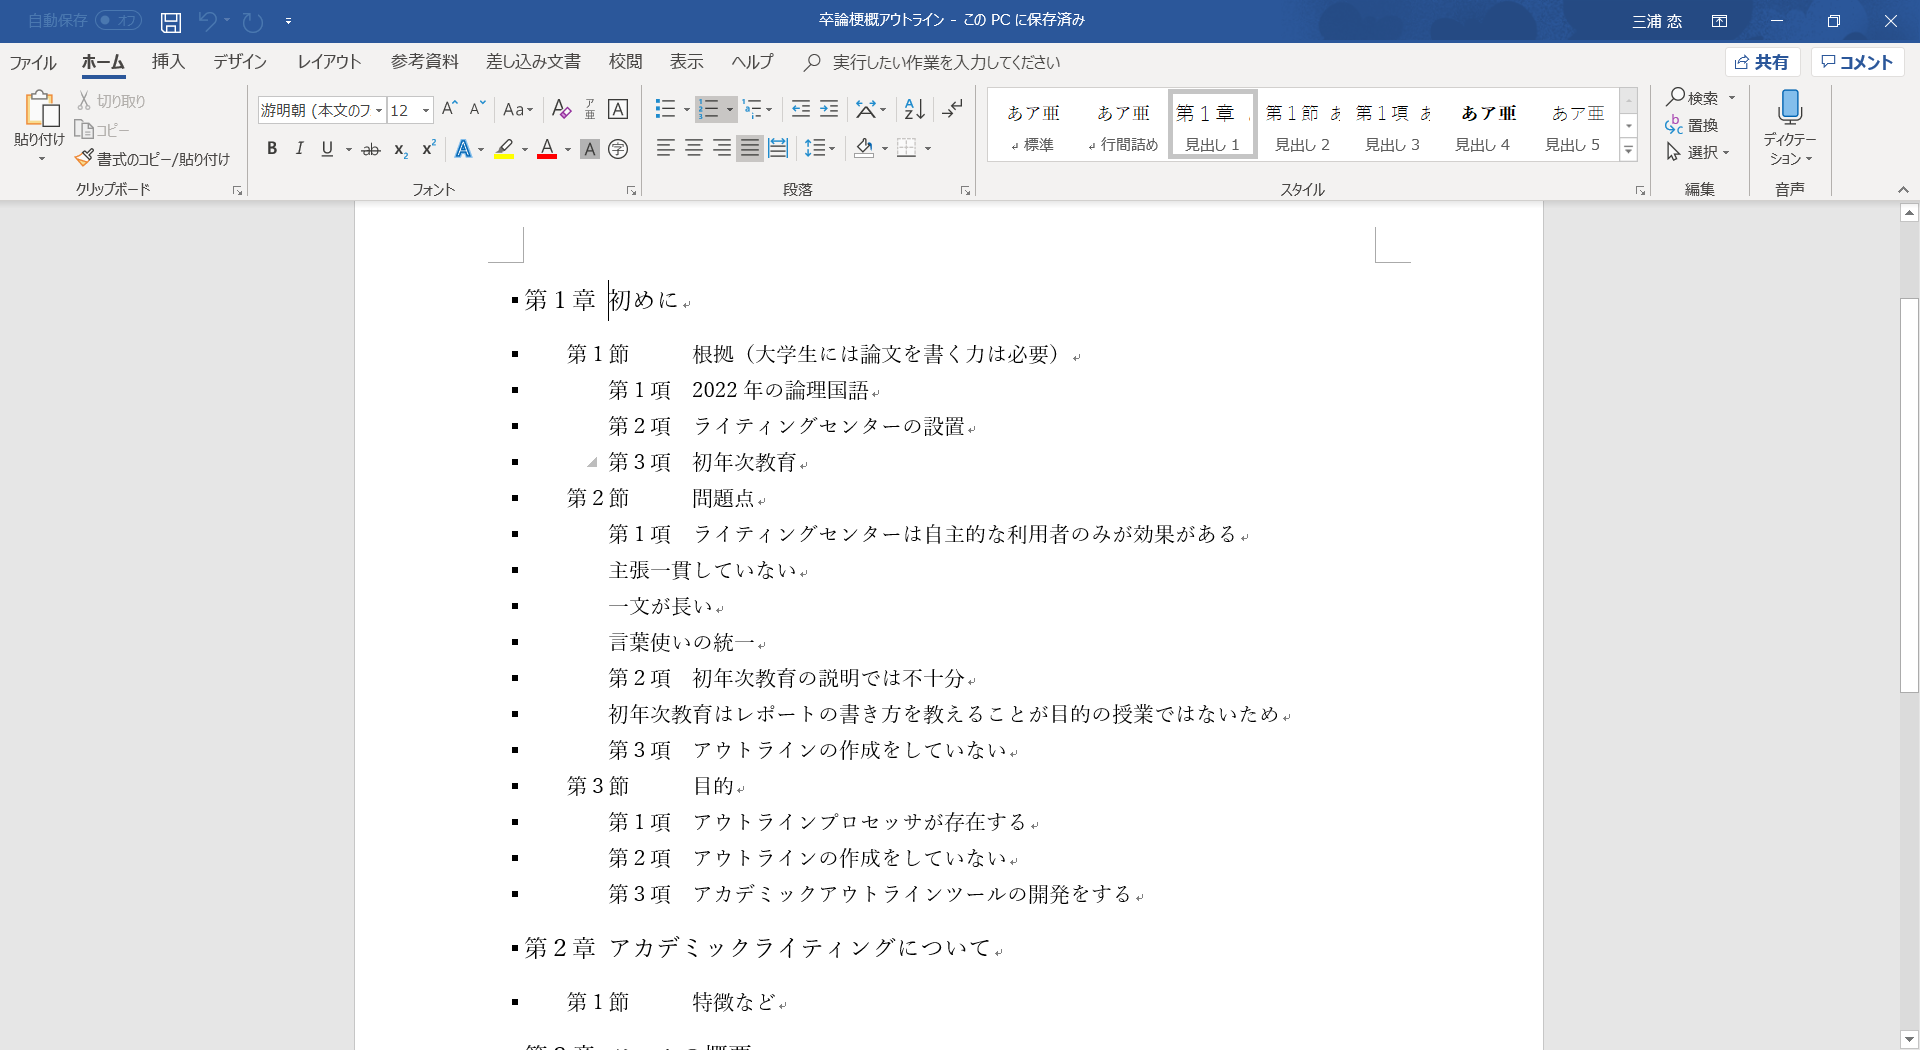
\includegraphics[clip,width=130mm,height=100mm]{word.png}
 \end{center}
 \caption{Microsoft Word}
 \label{fig:d}
\end{figure}

\newpage
\subsection{マインドマップ}
マインドマップとは,頭の中で自然に行っている思考のプロセスを反映したノート法である.イギリス人教育者であるトニー・ブザン (Tony Buzan)が1970年代に出演していたTV番組を始めとして様々な著作で「マインドマップ」という言葉が広め始めた\cite{ren4}.また,自由な思考,アイデアや情報の流れを中心となる概念から分岐させる形で描画した図である.描画することで,アイデアの整理,効果的なメモの作成,記憶の定着強化などを実現することが可能になる.実際のマインドマップの例としてSimple Mind liteを利用したものを図\ref{fig:e}に示す.
\begin{figure}[h]
\begin{center}
 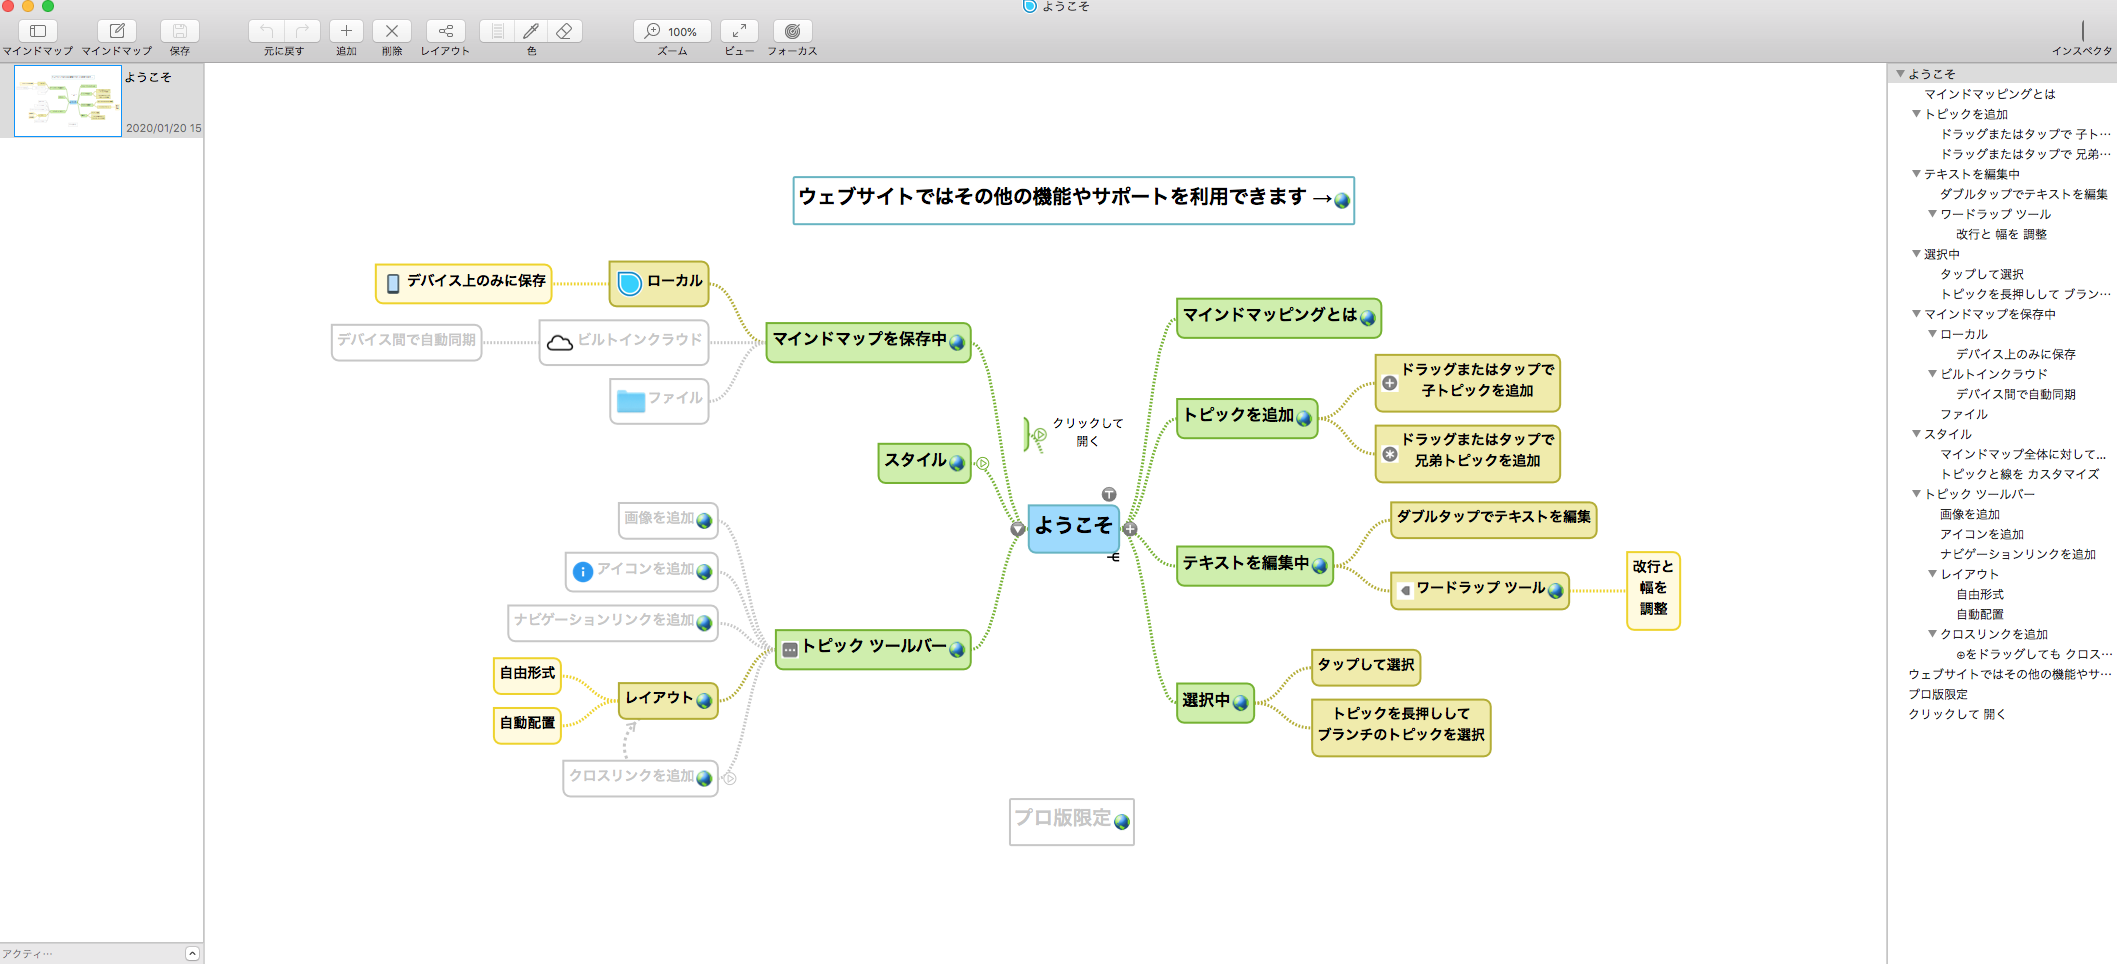
\includegraphics[clip,width=130mm,height=50mm]{maindmap.png}
\end{center}
 \caption{Simple Mind liteの使用例}
 \label{fig:e}
\end{figure}
\newpage

\newpage
\section{開発言語と関連技術}
開発言語として,自宅や学校のみならず隙間時間に利用することを視野に入れたため,PC とスマートフォンの両方からのアクセスによる利用を考えた.そこで Web 上で動作するツールが望ましいと考え,HTML5,CSS3, JavaScript を使用し開発を行った.
\subsection{HTML}
\subsubsection{HTMLについて}
HTMLとは,Hyper Text Markup Language の略称であり,ウェブ上のドキュメントを記述するためのマークアップ言語である.Webページを作成する際の基本的プログラミング言語であり,C言語の様なプログラミングとは異なり,文章中に記述することで様々な機能を設定することができる.HTMLでマークアップされたドキュメントは異なるドキュメントへのハイパーリンクを設定できるハイパーテキストであり,リスト,表等の高度な表現力も持ち合わせている.また,JavaScriptやCSSなどを直接書き込まなくても,別のファイルから呼び出すことが可能である\cite{ren8}.
\subsubsection{HTMLの特徴}
HTMLの特徴として,ハイパーテキストを利用した相互間文章参照のフレームワークが挙げられる.文章の特定要素にURIを用いた他文章へのリンクを記載することで,ユーザエージェントはそれを解釈し,指定された他文章を表示させることが可能である.マークアップは,プレーンテキストの文章を要素で括り意味づけすることで行うが,その際に引用する画像の埋め込みや文章タイトルの指定等を定める要素を記載することで,ユーザエージェントがそれらを解釈し見合った表示を行う\cite{ren8}.
\subsubsection{HTML5について}
HTML5とは,以前標準となっていたHTML4やXHTML1.xの後継にあたる使用である.しかし,HTML4やXHTML1.xが扱う範囲とは大きく異なり,範囲が多岐にわたることが特徴といえる.ここでは,マークアップの仕様だけでなく,周辺APIまで含めてHTML5と定義を行い,説明する.

HTML4やXHTML1.xではマークアップの仕様が主だったが,HTML5からマークアップだけでなく,DOMの仕様やAPIの仕様が数多く盛り込まれるようになった.これまでも多くのAPIが使用されてきたが,そのAPIは標準化団体であるW3Cが規定したAPIだけでなく,デファクトスタンダード化したAPIやブラウザベンダー独自のAPIが数多く使われてきた.このようなAPIはブラウザによって挙動が異なる,仕様書がないなどの問題があったが,HTML5で改めて仕様として規定し直されている.

また,CanvasやVideoなどのプラグインを用いなければ実現できなかった機能を,プラグインなしで実現できるようになり,File APIやWeb Workerの様なプラグインがあっても実現できなかった機能が開発された.これらのことから,HTML5はWebアプリケーションに必要とされる多くの要素を集結させた仕様であるといえる.

しかし,HTML4などで使用していた要素,属性などがいくつか廃止され,他の要素,属性を用いて使用する形になるなど,新しいものが追加されただけでなく,以前からあったものも多く変更がされているため注意が必要である\cite{ren8}.
\subsection{CSS}
\subsubsection{CSSについて}
CSSとはCascading Style Sheet の略称であり,HTMLなどのウェブページのスタイルを指定するための言語である.ウェブページをデザインする際のスタイルシート言語の1つであり,CSSが一般的に利用されている.ウェブページに書かれた各要素の装飾を指定することができ,スクリーンに表示される色やサイズ,レイアウトなどをCSSで指定することが可能である.
\subsubsection{CSS3について}
CSS3とは単一の規格ではなく,「CSS Color Module Level3」など機能単位で策定される方針に変更されたため,それらを総称してCSS3と呼ばれている.
\subsection{JavaScript}
\subsubsection{JavaScriptとは}
Netscape Communications社が開発した,プロトタイプベースのオブジェクト指向スクリプト言語である.Webブラウザにおいて,従来は印刷物のような静的な表現しかできなかったWebページに動きや対話性を付加することを目的に開発され,主要なWebブラウザに搭載された.しかし,各社の実装には微妙な違いがあり,Webブラウザによって使えない機能や,同じプログラムでも挙動が異るなどの問題があった.そのため,国際標準化団体であるEcmaインターナショナルによって中核的な仕様がECMAScriptとして標準化された.

Webブラウザと統合しているJavaScriptの処理系ではDOM(Document Object Model)操作が規定されており,動的なHTMLの構築を可能としている.この機能はAjaxの中核技術としても使われており,現在のWebアプリケーション開発に不可欠なものとなっている.

以前はインタプリタ方式で実行されることが一般的であったため,実行速度はさほど速くなかった.現在ではJITコンパイルなどを利用した各種の最適化がなされており,各Webブラウザベンダーともに高速化を図ってしのぎを削っている.
処理系の高速化やWebWorkersやWebGLなどの新しくAPIの追加により,Webブラウザ上で高度な計算や3DCGの描画など高度な処理が可能となっている\cite{ren9}.

\subsection{PWAについて}
PWA(Progressive Web Apps)とはモバイルサイト上でネイティブアプリのようなユーザー体験を提供する技術であり,ウェブとアプリの両方の良さを兼ね備えている.具体的にはインストールが必要なく,ホーム画面へのアイコン追加やプッシュ通知の可能であり,ユーザーとの接触機会を増やすことができる.また読み込み速度や表示の高速化,オフラインでの閲覧も可能であるなど様々なメリットが得られる.またアプリとの違いとして,アプリストアを経由してダウンロードやインストールする手間がなく,アプリの導入までの手順を短縮ができる.またプラットフォームごとに開発する必要もなく1つのPWAを構築するだけで,デバイスを問わずに一貫した内容を表示できるなど開発の自由度が高いことが特徴として言える\cite{ren6}.PWAの利用例として,図\ref{fig:f}に示す.
\begin{figure}[h]
\begin{center}
 \includegraphics[clip,width=150mm,height=80mm]{PWAgamen.pdf}
\end{center}
 \caption{PWAの例}
 \label{fig:f}
\end{figure}
\newpage

\section{本研究で開発したツールの概要}
\subsection{実装理由}
%実装した機能がなぜひつようであるのか?コンセプトを書く
本制作では論理的文章を書く際の準備段階である,アウトラインの作成をにおいて主張と根拠の確認や参考文献の管理を行うことでアウトラインの作成や主張の一貫した文章の作成を支援することができるツールが必要であると考えた.また,通学時間などの隙間時間で意見や構成の整理を行うことでアウトラインの作成時間を短くし,論理的文章を書く時間の確保ができることを目指した.

\subsection{実装した機能について}
本制作で開発したツールの機能は以下の4つである.ツール画面と機能\textcircled{\scriptsize 1}〜\textcircled{\scriptsize 4}の対応したものを図\ref{fig:g}に示す.
\begin{description}
  \item[\textcircled{\scriptsize 1}]主張と根拠の明確化
  \item[\textcircled{\scriptsize 2}]課題に対する疑問とその答えの記入
  \item[\textcircled{\scriptsize 3}]論理的な構成の整理
  \item[\textcircled{\scriptsize 4}]参考文献の管理
 \end{description}
%実際の画面を画像としてはる

\subsubsection{主張と根拠の明確化}
主張と根拠の明確化の機能は,アウトライン作成時に主張や根拠を表示させることで,アウトラインの作成や文章作成の際に確認を行い,主張からずれた意見が出ることを防ぐことができると考えこのような機能にした.
主張のテキストボックス内では課題に対した自分の主張を記入し,根拠のテキストボックスでは,下調べを行った際根拠となるものを記入する.

\subsubsection{課題に対する疑問とその答えの記入}
この機能では文章をアカデミックライティングの特徴である「問いと答え」の形式で記述を行うことで,文章に必要な情報などを明確化していくことができると考えこのような機能にした.また記入する内容としては,課題のテーマに対しての疑問とそれに対する自分の考えである答えをそれぞれ「問い」と「答え」の部分に記入してく.

\subsubsection{論理的な構成の整理}
この機能では,一般的なアウトラインプロセッサと同様に論理的な文章を書く上で各内容の順番や情報を整理するため順番を入れ替える機能,章や段落の情報を表示する機能にした.具体的にはボタンを押すことによって上下の内容が入れ替わる機能になっている.

\subsubsection{参考文献の管理}
文章を作成する際下調べなどで行った引用した文献や本などを確認,整理する機能にした.ここでは閲覧したサイトや検索した文献のWebページなどのURLを管理することや何章で扱う参考文献であるかを明確に表示することで参考文献の管理をしやすくするためこのような機能にした.
\newpage
\begin{figure}[h]
\begin{center}
 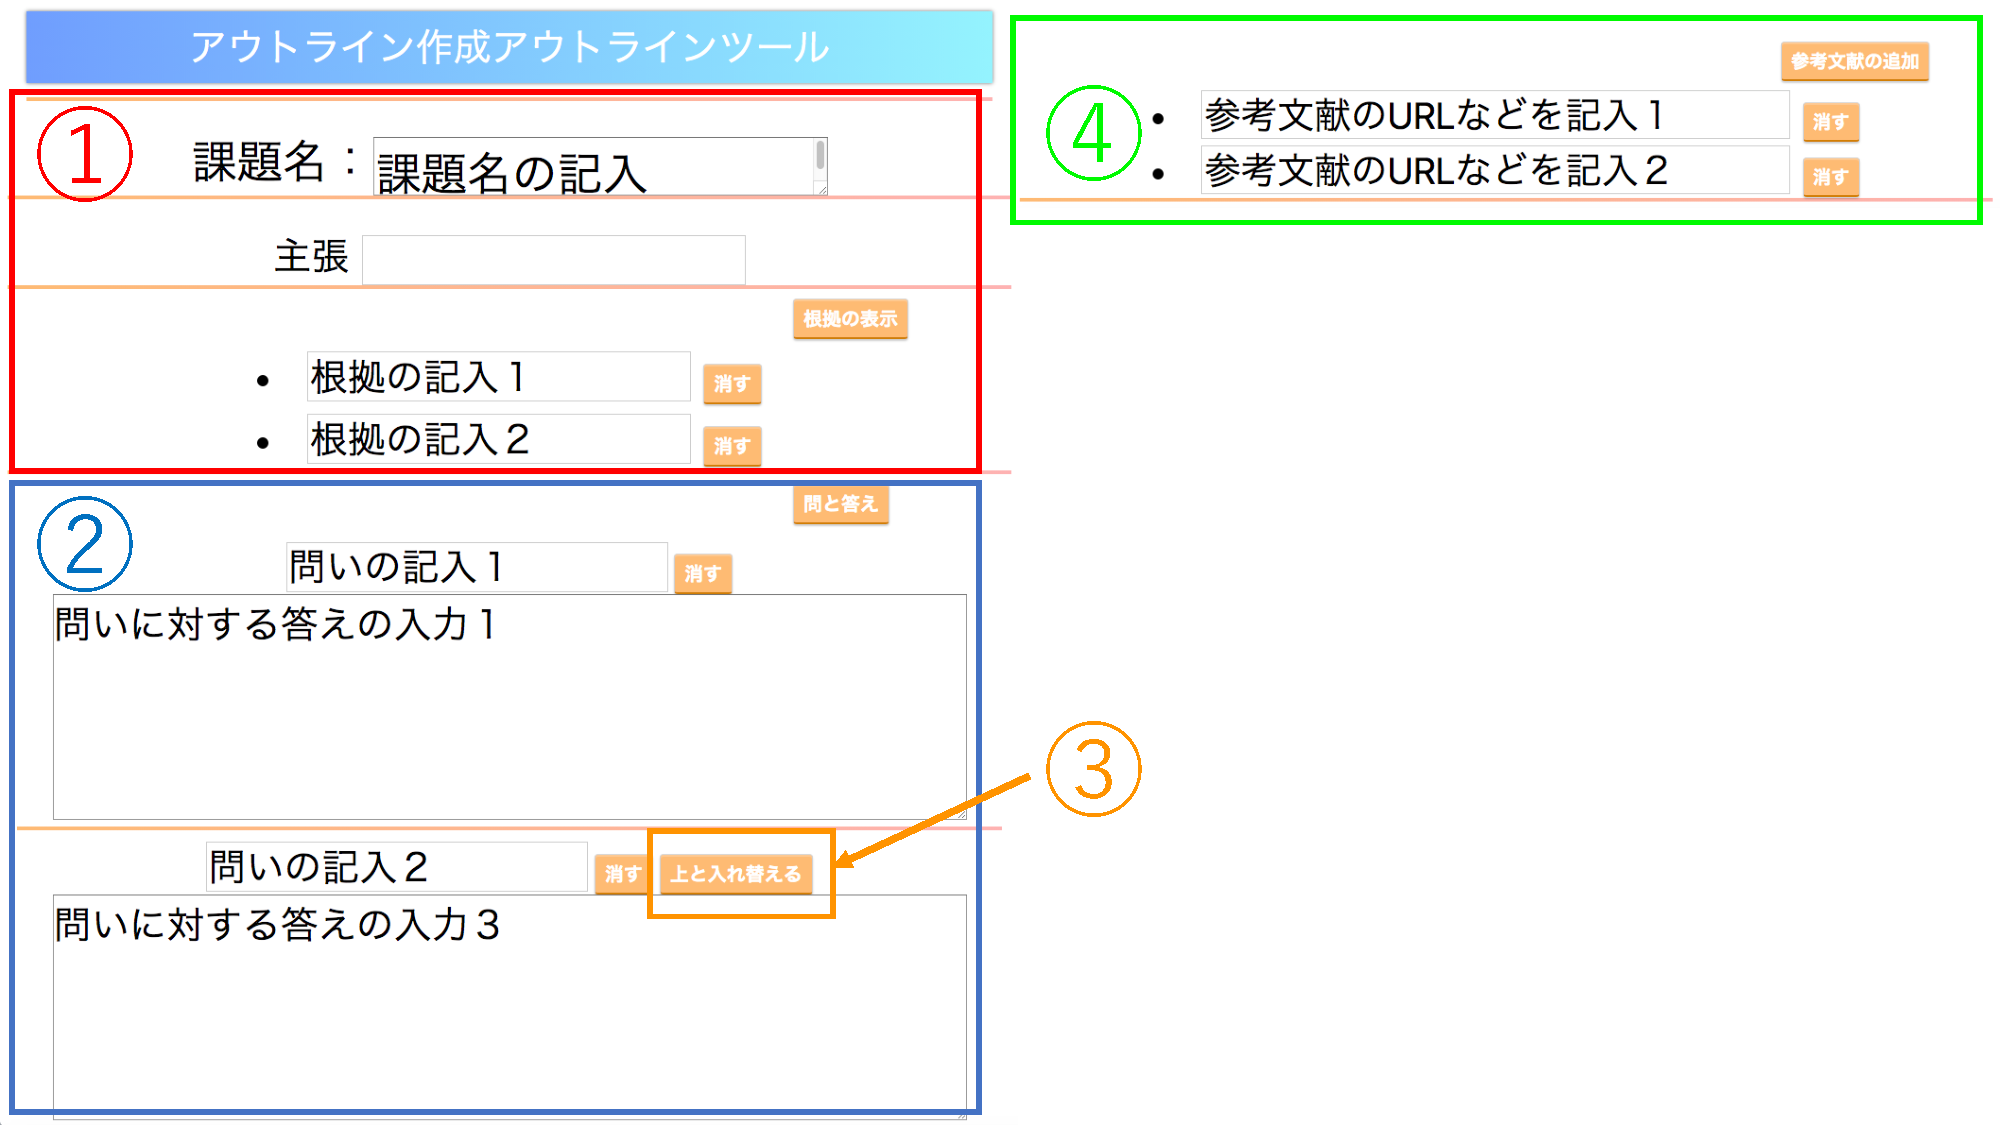
\includegraphics[clip,width=130mm,height=80mm]{pp01.pdf}
\end{center}
 \caption{アカデミックアウトラインツール}
 \label{fig:g}
\end{figure}
\newpage
\subsection{利用方法}
%図を使っての利用方法の説明を行う.
\subsubsection{課題名の記入欄}
図\ref{fig:h}は課題名の記入欄であり,論文のテーマやレポートの課題名などを記入する.
\begin{figure}[h]
\begin{center}
 
\includegraphics[clip,width=150mm,height=20mm]{00kadai.png}
\end{center}
 \caption{課題名の記入欄}
 \label{fig:h}
\end{figure}

\subsubsection{主張の記入欄}
図\ref{fig:i}は主張の記入欄であり,テーマや課題に対しての自分が考える主張を記入する.
\begin{figure}[h]
\begin{center}
 
\includegraphics[clip,width=150mm,height=15mm]{01shucho.png}
\end{center}
 \caption{主張の記入欄}
 \label{fig:i}
\end{figure}
\newpage
\subsubsection{根拠の記入欄}
根拠の表示のボタンを押すことで根拠を記入するテキストボックスが表示される.下調べを行った際の根拠となるものを記入していく.またアウトラインを作成し,整理していく中で不必要になったものがあった際には消すボタンでその根拠を消すことができる.表示前を図\ref{fig:j}に表示後を図\ref{fig:k}に示す.
\begin{figure}[h]
\begin{center}
 
\includegraphics[clip,width=150mm,height=10mm]{02konkyo.png}
\end{center}
 \caption{根拠の表示前}
 \label{fig:j}
\end{figure}

\begin{figure}[h]
\begin{center}
 
\includegraphics[clip,width=150mm,height=30mm]{03konkuo.png}
\end{center}
 \caption{根拠の表示後}
 \label{fig:k}
\end{figure}

\newpage
\subsubsection{問いと答えの記入欄}
問と答えのボタンを押すことで,問いの記入と答えの記入欄が表示される.テーマや課題に対しての疑問や何を論じるのかを問いの部分に記入をする.またそれに対応する答えを記入する.書いた文章の整理を行うため,上と入れ替えるボタンを押すことで上下のテキストボックス内のないよを入れ替えることができ,論理的なアウトラインの作成を支援することができる.表示前を図\ref{fig:l}に表示後を図\ref{fig:m}に示す.

\begin{figure}[h]
\begin{center}
 
\includegraphics[clip,width=150mm,height=10mm]{04qanda.png}
\end{center}
 \caption{問いと答えの表示前}
 \label{fig:l}
\end{figure}

\begin{figure}[h]
\begin{center}
 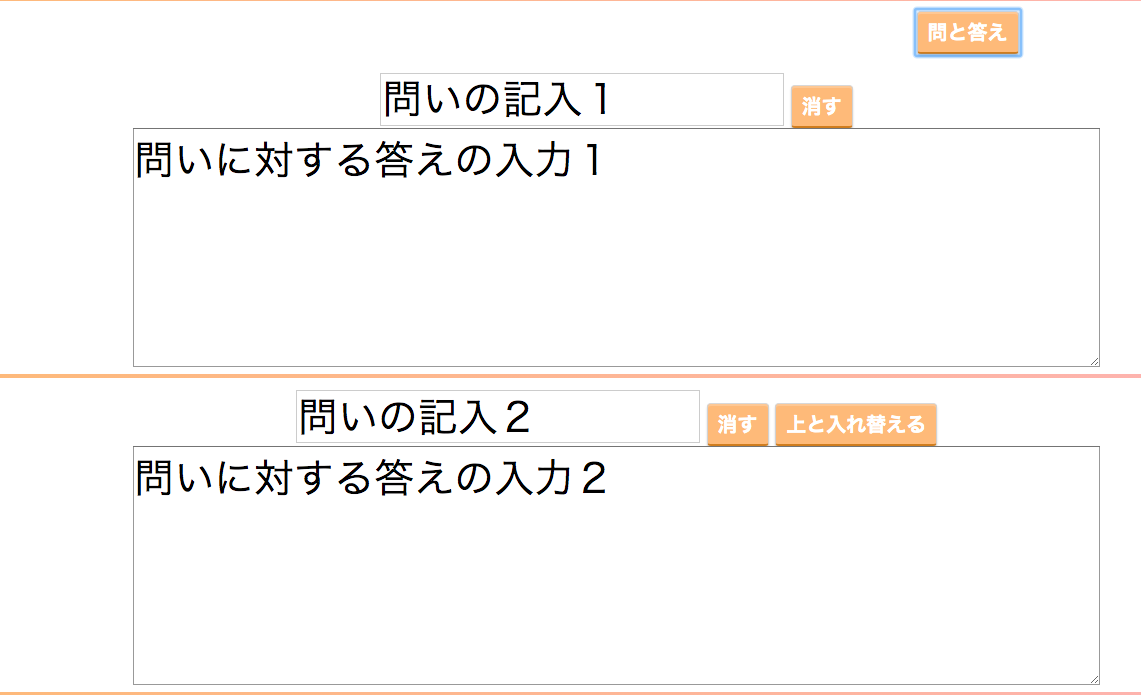
\includegraphics[clip,width=150mm,height=95mm]{05qanda.png}
\end{center}
 \caption{問いと答えの表示後}
 \label{fig:m}
\end{figure}
\newpage

\subsubsection{参考文献の管理}
参考文献のボタンを押すことで引用したサイトのURLなどを記入する欄が表示される.下調べの際に見た本やサイトを記入し管理をしておく.管理する際に何章で引用する文献なのか記入しておく.また参考文献の記入欄を追加する際は,参考文献のボタンをもう一度押すことで,記入欄が増える.表示前を図\ref{fig:n}に表示後を図\ref{fig:o}に示す.

\begin{figure}[h]
\begin{center}
 
\includegraphics[clip,width=150mm,height=10mm]{06sankou.png}
\end{center}
 \caption{参考文献の表示前}
 \label{fig:n}
\end{figure}

\begin{figure}[h]
\begin{center}
 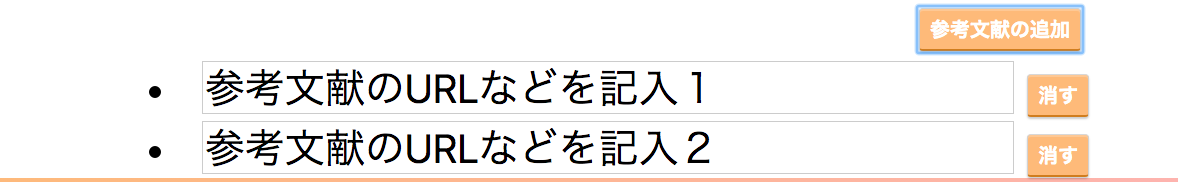
\includegraphics[clip,width=150mm,height=25mm]{07sankou.png}
\end{center}
 \caption{参考文献の表示後}
 \label{fig:o}
\end{figure}

\newpage
\subsection{画面構成について}
本ツールはPCでの作業だけでなく,移動時間などの隙間時間での利用も考えたため,スマートフォンでの利用もすることができる.そのため機能は変わらないがPC版とスマートフォン版とipad版の3種類に対応できるよう画面サイズに合わせた画面構成を行った.以下の図がそれぞれPC版を図\ref{fig:p},スマートフォン版とipad版を図\ref{fig:q}に示す.
\begin{figure}[h]
\begin{center}
 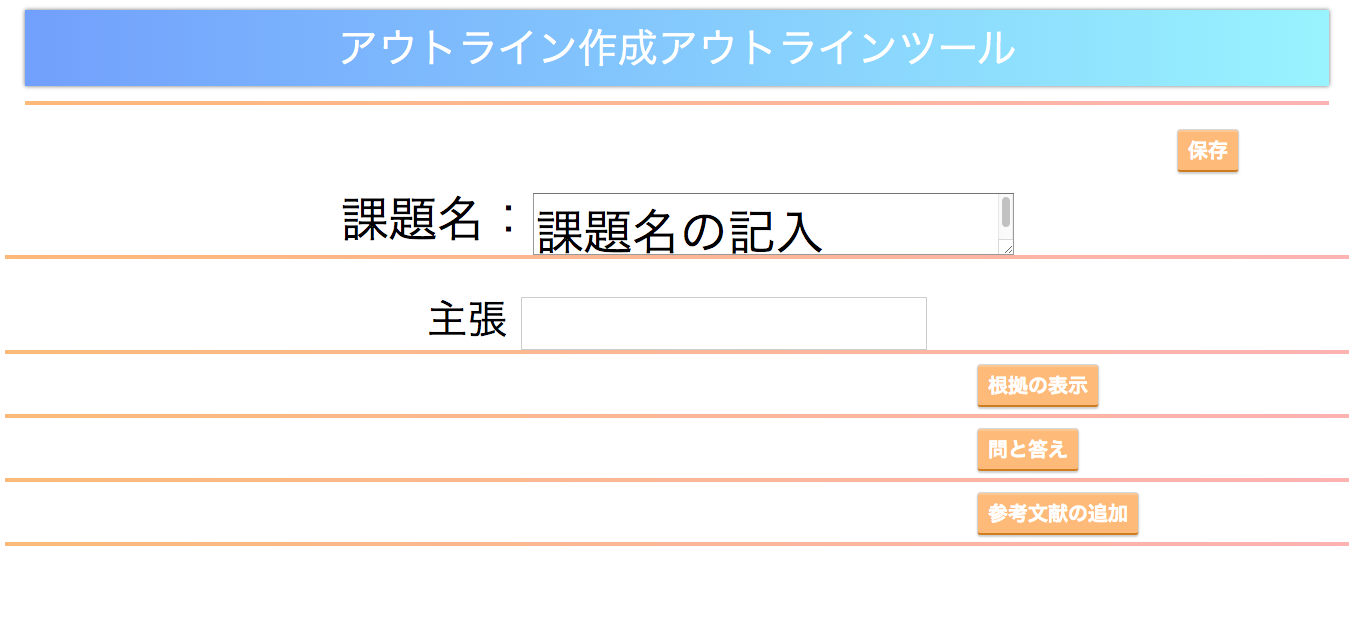
\includegraphics[clip,width=130mm,height=70mm]{08gamen.png}
\end{center}
 \caption{PC版}
 \label{fig:p}
\end{figure}

\begin{figure}[h]
\begin{center}
 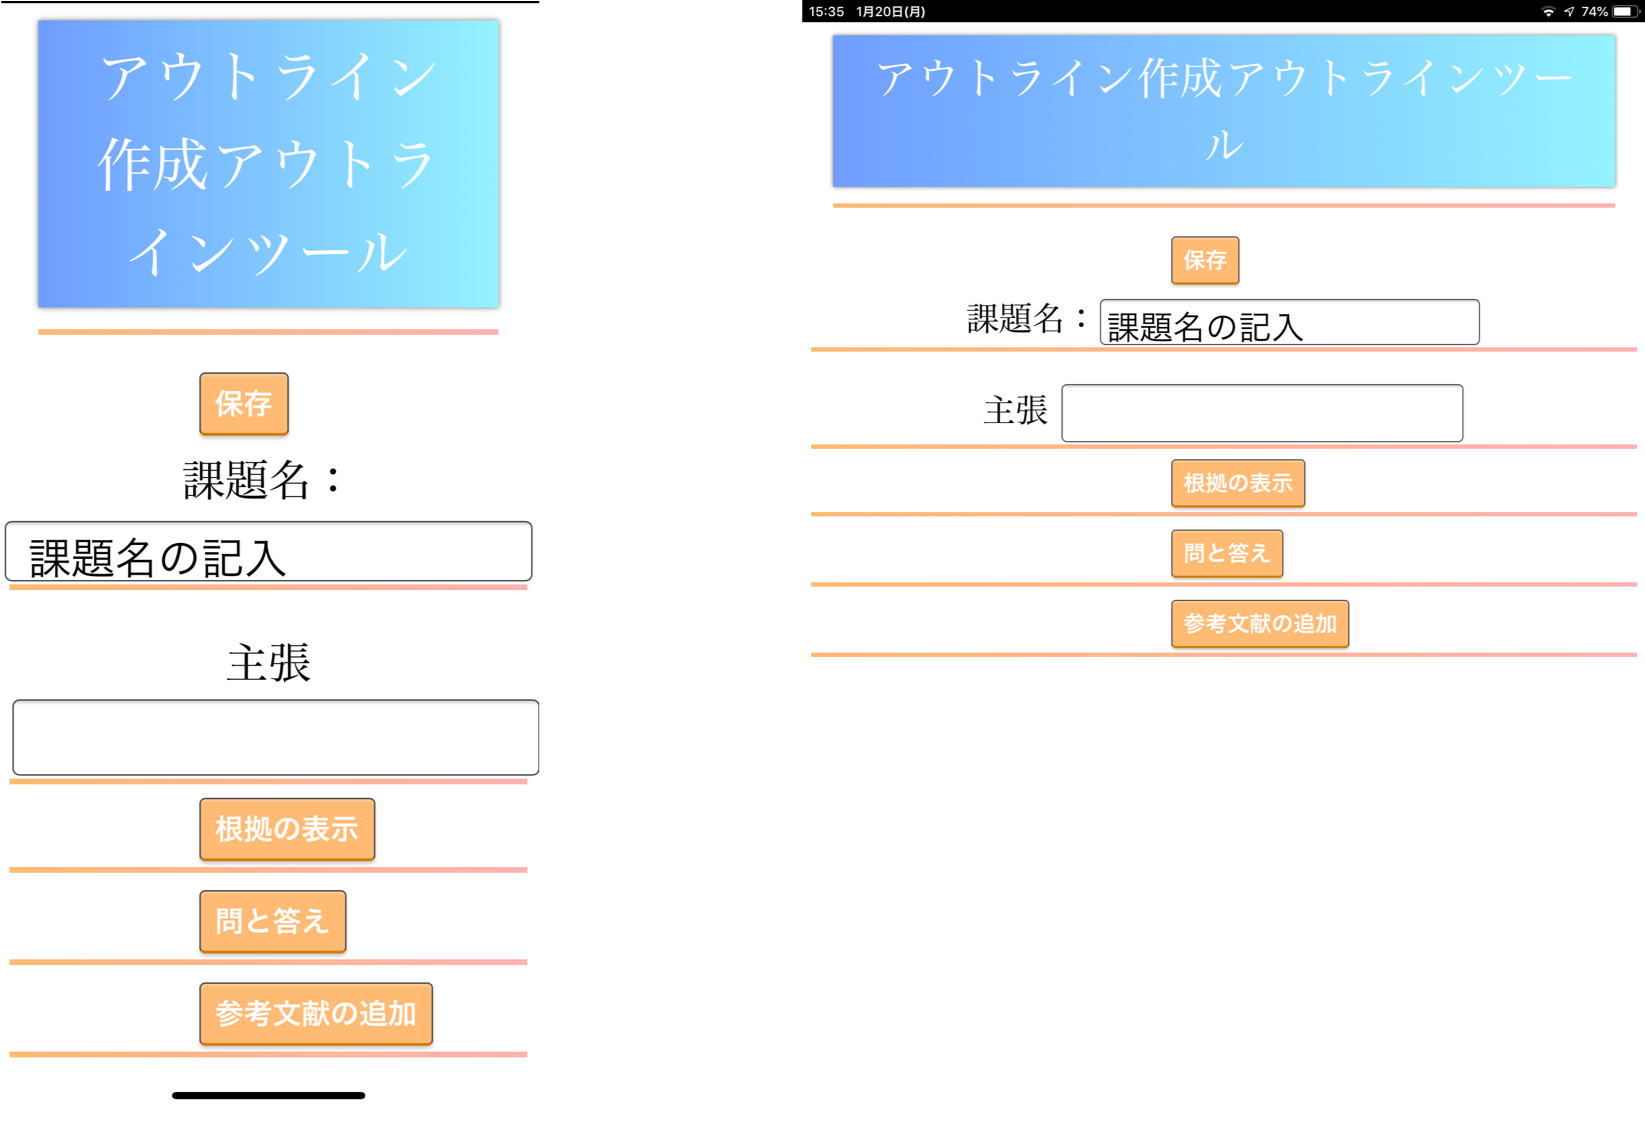
\includegraphics[clip,width=90mm,height=60mm]{17.png}
\end{center}
 \caption{スマートフォン版とipad版}
 \label{fig:q}
\end{figure}

\newpage
\section*{結言}
%背景
大学で論文やレポートを書かなければならない大学生に対して,論理的な思考力や論理的文章作成能力の要求が高まっている.しかし,論文やレポートを書く際にアウトラインなどの事前準備をせずに文章の作成を行ってしまう学生が多く,論理的な文章にならないことが問題点として挙げられる.
そのため,レポートの書き方の指導や修正を行うライティングセンターの設置などが進められているが継続的な利用が必要とされている.

%問題点
しかし,一般に論文や小説などの長文を作成を支援するためのツールとして,アウトラインプロセッサが使用されることが多い.
これは,文章を階層的に管理することに主眼が置かれており,学生にとって主張や根拠などが明確な一貫した文章を書く力を養うためのツールではないことが問題点となっている.

%目的
そこで本制作では,主張や根拠などが明確な一貫した論文やレポートを書くため,準備段階であるアカデミックアウトラインツールを開発することを目的としている.

%結果
本制作を行い論理的文章のアウトラインの作成を支援するツールの開発を行ったが,
\section*{謝辞}
\addcontentsline{toc}{section}{謝辞}
本制作の遂行および本論文の作成にあたり,多くの御助言とご指導を頂きました須田宇宙准教授に深く感謝の意を表します.
\bibliographystyle{jplain}

\addcontentsline{toc}{section}{参考文献}
 \begin{thebibliography}{99}
\bibitem{ren1}山崎 憲一,萬代 雅希:"論文とは",電子情報通信学会 通信ソサイエティマガジン,2016年9巻4号216-221.
\url{https://www.jstage.jst.go.jp/article/bplus/9/4/9_216/_pdf}

\bibitem{ren2} 堀 一成,坂尻 彰宏:"阪大生のためのアカデミックライティング",
\url{https://ir.library.osaka-u.ac.jp/repo/ouka/all/27153/Academic%20Writing%20Introduction.pdf}, 2019/8/23参照

\bibitem{ren7}早稲田ウィークリー:"アカデミック・ライティング力を磨こう",
\url{https://www.waseda.jp/inst/weekly/feature/2014/06/23/20860/}

\bibitem{ren3} 山本 浩: "TeXを使った論文作成方法",2000年103巻984号770-773.
\url{https://www.jstage.jst.go.jp/article/jsmemag/103/984/103_KJ00001459868/_article/-char/ja/}

\bibitem{ren4} Lucidchart:"5分でわかる、マインドマップの書き方と意味",\url{https://www.lucidchart.com/pages/ja/mind-map#section_0}

\bibitem{ren5} マインドマップの学校:"マインドマップの書き方・描き方「6つの法則」",\url{https://www.mindmap-school.jp/mindmap/mindmap-law/}

\bibitem{ren6} ディーエムソリューションズ株式会社:"PWAとは?メリットと実装例について"\url{https://digital-marketing.jp/seo/what-is-progressive-web-apps/#i-6}

\bibitem{ren8}大嶋 泰史:"HTML5に対応した仮想座標グラフィックライブラリの構築",千葉工業大学卒業論文,2012
\bibitem{ren9}田口 優希: "MeSH拡張のためのサーバ感通信アーキテクチャ", 千葉工業大学卒業論文,2012

\end{thebibliography}
\newpage
\section*{付録}

\addcontentsline{toc}{section}{付録}

\end{document}
